\section{Illustrations of the actual dual-comparison
continuation}\label{illustrations-of-the-actual-dual-comparison-continuation}

\begin{figure}
\centering
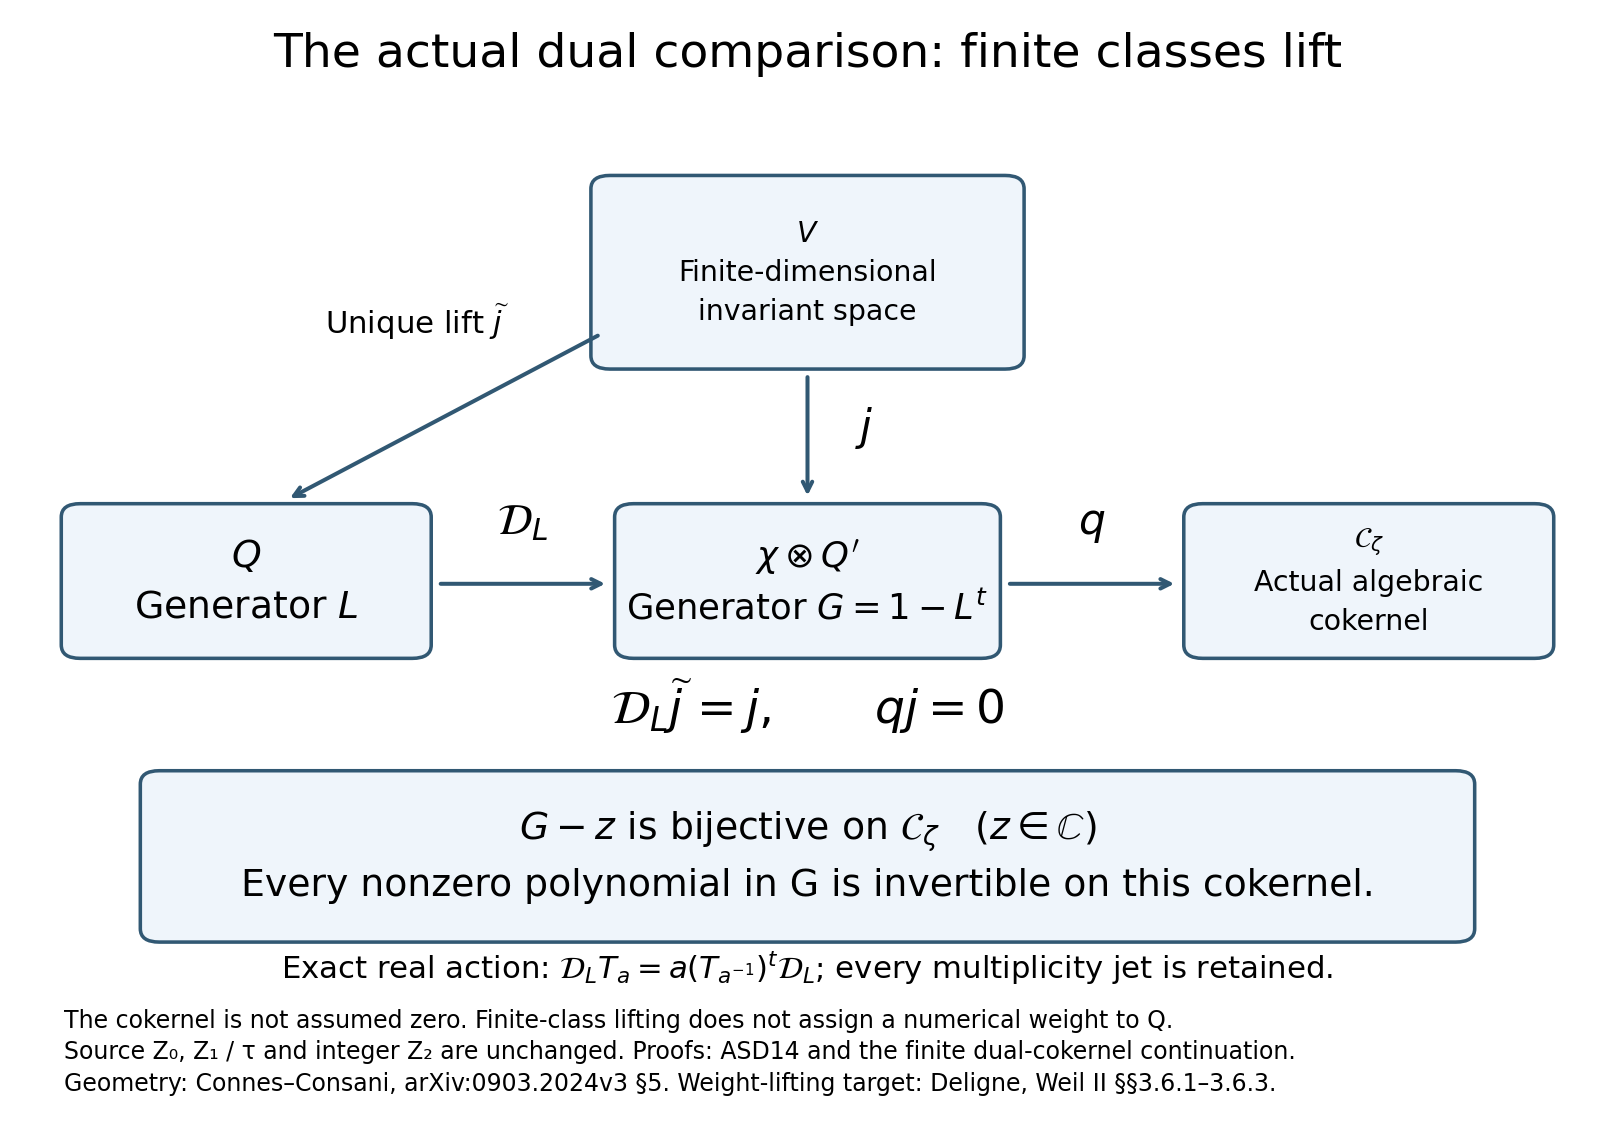
\includegraphics[width=\textwidth,height=.83\textheight,keepaspectratio]{tau_lifting_weights_20260924/FINITE_DUAL_LIFT.png}
\caption{Finite classes lift}
\end{figure}

Figure 1. Complete proofs:
\href{SPECTRAL_COKERNEL_DIVISIBILITY_AND_FINITE_LIFTING.md}{SCL2--SCL9}
and
\href{DUALITY_COKERNEL_POLYNOMIAL_LIFTING_INDEPENDENT.md}{DPL1--DPL9}.
The actual target is the character-a-twisted continuous dual, with
generator G=1−L\^{}t. The upper space is finite-dimensional and
invariant for the specified receiving action; its lift is unique. The
whole algebraic cokernel is retained. This picture assigns no weight or
parity to primitive tau.

\begin{figure}
\centering
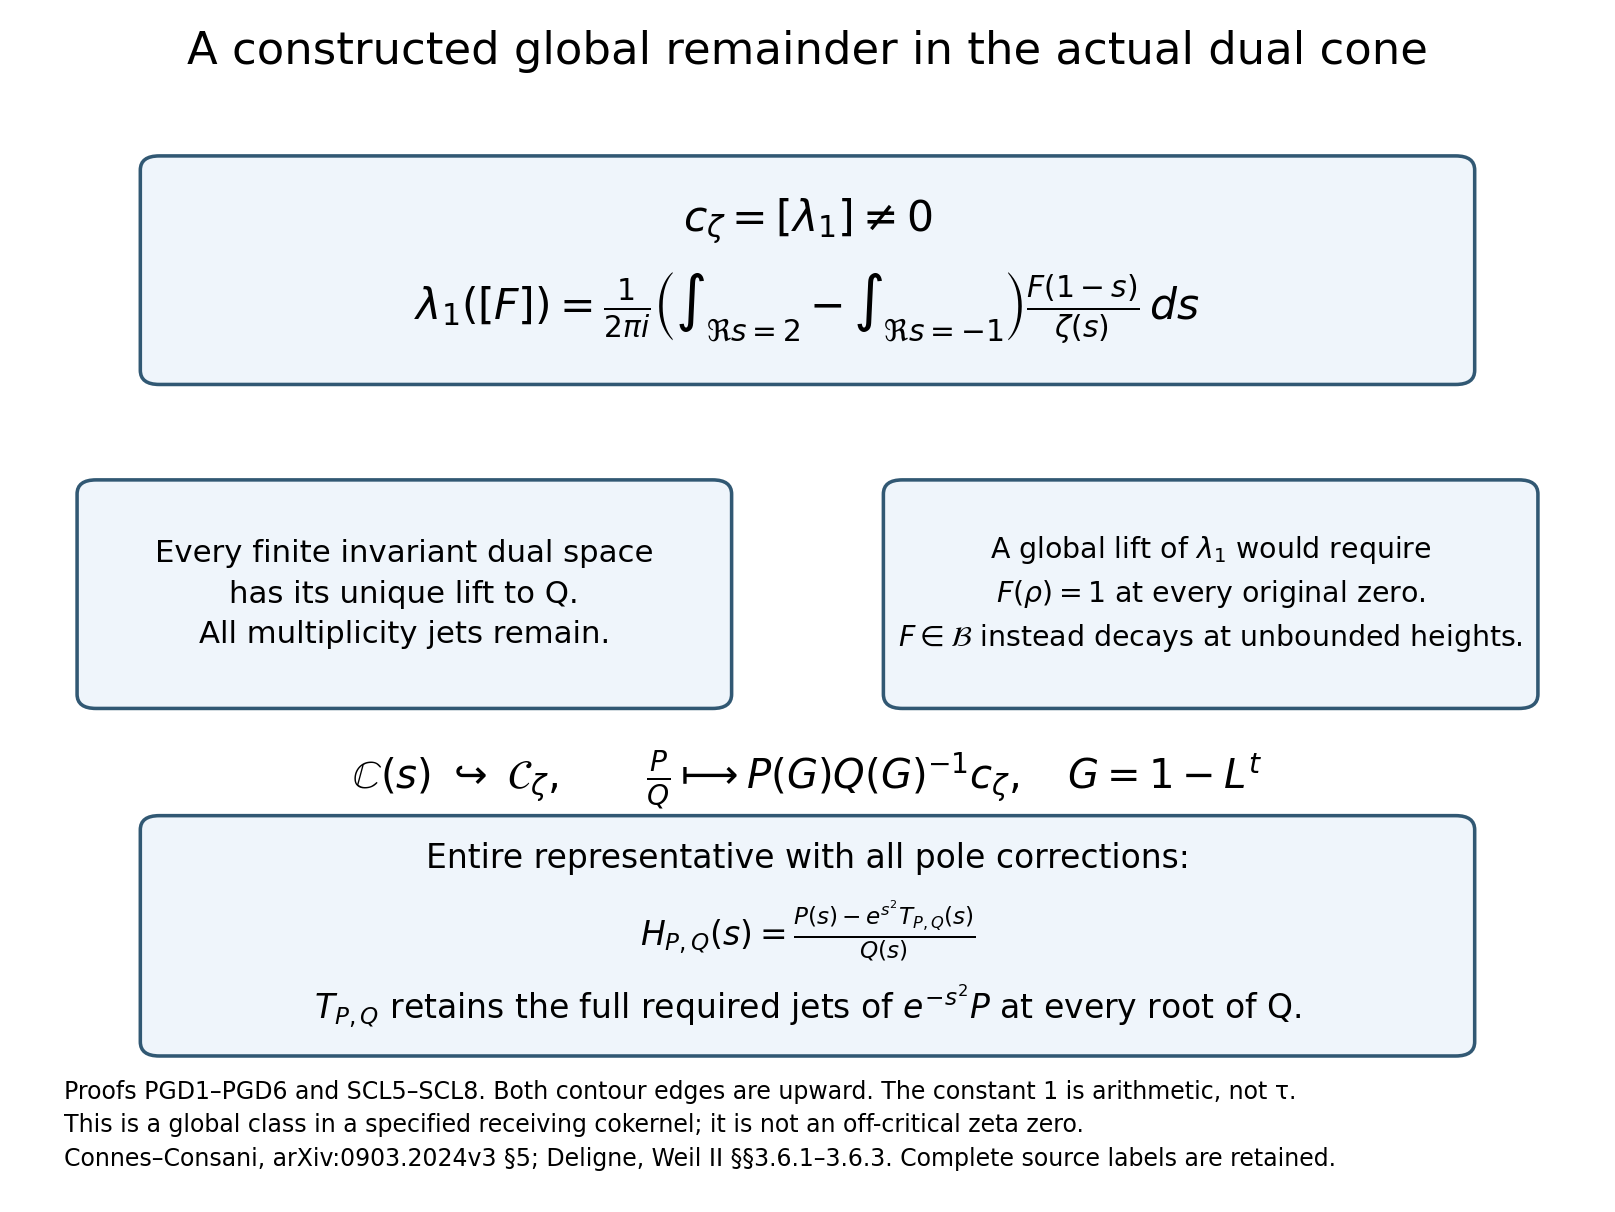
\includegraphics[width=\textwidth,height=.83\textheight,keepaspectratio]{tau_lifting_weights_20260924/GLOBAL_POLYNOMIAL_DUAL_DEFECT.png}
\caption{The explicit global remainder}
\end{figure}

Figure 2. Complete proof:
\href{GLOBAL_POLYNOMIAL_DUAL_DEFECT.md}{PGD1--PGD6}; independent
verification
\href{GLOBAL_POLYNOMIAL_DUAL_DEFECT_INDEPENDENT_CHECK.md}{PGC0--PGC7}.
Both contour edges point upward. All original-zeta factors, multiplicity
jets, and the rational representative's entire correction are retained.
The polynomial T has the exact prescribed derivatives of orders 0
through k−1 at every denominator root of multiplicity k. The arithmetic
constant1 is not primitive tau. The class is not a claimed RH
counterexample.

Reproducible sources: check\_and\_draw\_finite\_dual\_lift.py, with SVG
files beside these PNGs. The 36 finite symbolic checks supplement the
complete global analytic proofs. Both final figures were inspected and
their spacing corrected.

Human sources: Alain Connes and Caterina Consani,
\href{https://arxiv.org/abs/0903.2024v3}{Schemes over F1 and zeta
functions}, §5; Ralf Meyer,
\href{https://arxiv.org/abs/math/0412277v3}{Spectral interpretation};
Pierre Deligne,
\href{https://www.numdam.org/item/PMIHES_1980__52__137_0/}{Weil II},
§§3.6.1--3.6.3; Hadamard's product through the indexed original
\href{https://arxiv.org/abs/2602.04022v1}{Connes treatment}. Exact
versions, source files and actual reading coverage remain in
\nolinkurl{SOURCE_READING_USE_PRIVATE.json}.
